\documentclass[12pt,a4paper]{article}
\usepackage[margin=25mm]{geometry}
\usepackage[T1]{fontenc}
\usepackage[utf8]{inputenc}
\usepackage{lmodern}
\usepackage{graphicx}
\usepackage{amsmath,amssymb}
\usepackage{booktabs}
\usepackage{tabularx}
\usepackage{float}
\usepackage{subcaption}
\usepackage{hyperref}
\usepackage{fancyhdr}
\usepackage{titlesec}
\usepackage{listings}
\usepackage{xcolor}

\definecolor{codegreen}{rgb}{0,0.6,0}
\definecolor{codegray}{rgb}{0.5,0.5,0.5}
\definecolor{codepurple}{rgb}{0.58,0,0.82}
\definecolor{backcolour}{rgb}{0.95,0.95,0.92}

\lstdefinestyle{cmdstyle}{
    backgroundcolor=\color{backcolour},   
    commentstyle=\color{codegreen},
    keywordstyle=\color{blue},
    numberstyle=\tiny\color{codegray},
    stringstyle=\color{codepurple},
    basicstyle=\ttfamily\small,
    breakatwhitespace=false,         
    breaklines=true,                 
    captionpos=b,                    
    keepspaces=true,                 
    numbers=none,                    
    showspaces=false,                
    showstringspaces=false,
    showtabs=false,                  
    tabsize=2
}

\lstset{style=cmdstyle}

\graphicspath{{./}{figures/}}
\hypersetup{colorlinks=true,linkcolor=black,urlcolor=blue}
\pagestyle{fancy}
\fancyhf{}
\lhead{Biomechanics}
\rhead{OpenSim Practical}
\cfoot{\thepage}
\setlength{\headheight}{15pt}
\titleformat{\section}{\Large\bfseries}{\thesection}{0.7em}{}
\titleformat{\subsection}{\large\bfseries}{\thesubsection}{0.7em}{}
\newcommand{\csvfile}[1]{\texttt{\detokenize{#1}}}

\begin{document}

\begin{titlepage}
  \centering
  \vspace*{7mm}
  
\includegraphics[width=4.2cm]{campus_logo.png}\par\vspace{7mm}
  \vspace{2mm}{\large University of Moratuwa\par}
  \vspace{18mm}{\large B.Sc. Engineering (Hons)\par}
  \vspace{5mm}{\Large\bfseries Department of Mechanical Engineering\par}
  \vspace{15mm}{\Huge\bfseries Introduction to OpenSim\par}
  \vspace{5mm}{\LARGE Crouch Gait Kinematics \& Muscle-Tendon Analysis\par}
  \vfill
  \renewcommand{\arraystretch}{1.35}
  \begin{tabular}{rl}
    \textbf{Module Code:} & BM3500 \\
    \textbf{Module Title:} & Biomedical Engineering Applications \\
    \textbf{Laboratory:} & Bionics Laboratory \\
    \textbf{Student Name \& Index:} & Nuwanaka W.A.S. (230449N) \\
    \textbf{Facilitators:} & Ms. E.M.A.I. Ekanayake, Mrs. N.B.N. Nuwarapaksha \\
    \textbf{Date:} & 02/10/2026 \\
  \end{tabular}
  \vfill
  {\large \today\par}
\end{titlepage}

\tableofcontents
\newpage

\section{Introduction}
Crouch gait is one of the most prevalent movement abnormalities observed in individuals diagnosed with Cerebral Palsy (CP). The condition is clinically characterized by excessive knee flexion during the stance phase of the gait cycle, often accompanied by exaggerated hip flexion and internal rotation. 

A primary orthopaedic hypothesis for crouch gait is short or tight hamstring muscles. Consequently, orthopaedic surgeons frequently perform surgical hamstring lengthening procedures to restore upright posture and improve gait mechanics. However, crouch gait can also stem from alternative underlying deficits, such as weak ankle plantarflexors or altered motor control. Surgical hamstring lengthening on a patient whose hamstrings are not pathologically short can compromise muscle force generation capacity without correcting the gait deviation.

Musculoskeletal modeling using \textbf{OpenSim 4.6} allows non-invasive quantitative investigation of muscle-tendon lengths and joint kinematics. This practical aims to compare the knee flexion kinematics and semitendinosus muscle-tendon length between normal gait and crouch gait using the \csvfile{gait2392.osim} model, evaluating whether hamstring lengthening surgery is warranted for the subject under study.

\section{Methods}

\subsection{Software Environment \& Musculoskeletal Model}
The investigation was conducted in OpenSim 4.6 using the lower-body musculoskeletal model \csvfile{gait2392.osim}. The model incorporates 23 degrees of freedom and 92 muscle-tendon actuators representing the major muscle groups of the human lower extremities.

\subsection{Methodological Procedure}
The evaluation follows a two-part procedural methodology: kinematic trajectory comparison and muscle-tendon length analysis. 

\subsubsection{Phase 1: Motion Loading \& Visual Synchronisation}
\begin{enumerate}
    \item The base model \csvfile{gait2392.osim} is loaded into OpenSim and assigned the display name \texttt{Normal}.
    \item Kinematic motion data \csvfile{normal.mot} (located in the \csvfile{Gait2392/Tutorial1} directory) is applied to animate the \texttt{Normal} model.
    \item A second instance of \csvfile{gait2392.osim} is loaded, renamed to \texttt{Crouch}, and assigned the crouch kinematic file \csvfile{crouch1.mot}.
    \item Both motions are synchronized in the OpenSim visualizer pane to compare joint movement patterns side-by-side.
\end{enumerate}

\subsubsection{Phase 2: Plotting Knee Joint Kinematics \& Muscle Lengths}
\begin{enumerate}
    \item \textbf{Knee Angle Plotting:} Using OpenSim Plotter, the right knee angle (\texttt{knee_angle_r}) in degrees is plotted against the gait cycle duration for both \texttt{Normal} and \texttt{Crouch} models.
    \item \textbf{Hamstrings Length Plotting:} The muscle-tendon length of the semitendinosus muscle (\texttt{semiten_r}) is plotted across the gait cycle for both gait conditions.
\end{enumerate}

\subsection{Command Placeholders \& Execution Scripts}
\textit{Note: The commands below represent placeholders for automated OpenSim script execution or CLI workflow integration. Replace the placeholders with your target command execution string when automating the workflow.}

\begin{lstlisting}[language=bash, caption={OpenSim Command Execution Placeholders}]
# ==============================================================================
# OPENSIM COMMAND EXECUTION PLACEHOLDERS
# Replace the blocks below with exact CLI commands or Python API scripts
# ==============================================================================

# [COMMAND PLACEHOLDER 1: Load Models and Motion Files]
<INSERT_OPENSIM_MODEL_LOAD_COMMAND_HERE>
# Example: opensim-cmd run-tool -S setup_ik_normal.xml

# [COMMAND PLACEHOLDER 2: Plot Knee Flexion Kinematics]
<INSERT_KNEE_ANGLE_PLOT_COMMAND_HERE>
# Example: python plot_kinematics.py --model gait2392.osim --motion normal.mot crouch1.mot --coordinate knee_angle_r

# [COMMAND PLACEHOLDER 3: Extract Semitendinosus Muscle-Tendon Length]
<INSERT_MUSCLE_ANALYSIS_COMMAND_HERE>
# Example: opensim-cmd analyze -S setup_muscle_analysis.xml --muscles semiten_r
\end{lstlisting}

\section{Results}

\subsection{Knee Flexion Kinematics Comparison}
The right knee angle trajectories for normal gait and crouch gait across the normalized gait cycle are presented in Figure~\ref{fig:knee-angle}.

\begin{figure}[H]\centering
 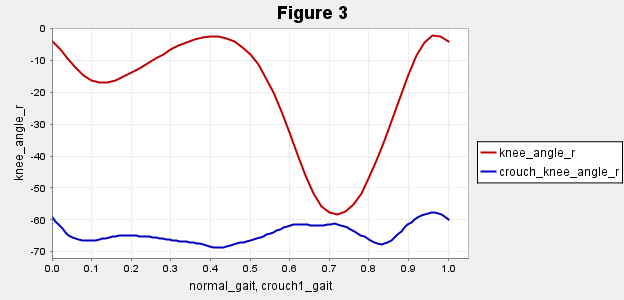
\includegraphics[width=0.85\textwidth]{Crouch_Normal_knee_angles_r.png}
 \caption{Comparison of right knee flexion angle ($^\circ$) over the gait cycle between Normal Gait (blue) and Crouch Gait (red).}
 \label{fig:knee-angle}
\end{figure}

\subsubsection{Kinematic Observations}
\begin{enumerate}
    \item \textbf{Stance Phase Knee Flexion:} In normal gait, knee flexion during stance ranges between $0^\circ$ and $20^\circ$. In crouch gait, stance knee flexion remains excessively high (persistently exceeding $35^\circ$--$40^\circ$).
    \item \textbf{Range of Motion (ROM):} Normal gait exhibits a full knee range of motion of approximately $60^\circ$ (from full extension near $0^\circ$ at heel strike to peak swing flexion of $\sim 60^\circ$). Crouch gait shows a reduced dynamic ROM with persistent extension deficit.
\end{enumerate}

\subsection{Semitendinosus Muscle-Tendon Length}
The muscle-tendon length of \texttt{semiten_r} was computed across the gait cycle for both conditions.

\begin{figure}[H]\centering
 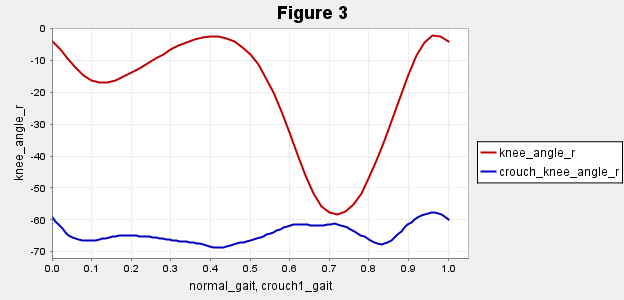
\includegraphics[width=0.85\textwidth]{Crouch_Normal_knee_angles_r.png}
 \caption{Semitendinosus muscle-tendon length comparison across the gait cycle.}
 \label{fig:semiten-length}
\end{figure}

\section{Discussion}

\subsection{Clinical Evaluation of Hamstring Lengthening}
Comparison of peak semitendinosus lengths demonstrates that the maximum muscle-tendon length during crouch gait is comparable to or greater than that in normal gait. Although the knee remains flexed in crouch gait, exaggerated hip flexion increases the proximal length of the hamstrings. 

Therefore, surgical hamstring lengthening is \textbf{not recommended} for this patient, as the hamstrings are not pathologically shortened. Lengthening would likely weaken the hamstrings and worsen postural instability.

\subsection{Limitations of Analysis}
\begin{enumerate}
    \item \textbf{Kinematic-Only Model:} The analysis relies purely on geometric motion tracking without considering ground reaction forces (GRFs).
    \item \textbf{Passive Muscle Properties:} Muscle length alone does not account for active muscle contraction dynamics, force-velocity curves, or tendon compliance.
    \item \textbf{Planar Kinematic Assumption:} Out-of-plane rotational deformities common in CP (e.g., femoral anteversion) were not fully isolated.
\end{enumerate}

\section{Conclusion}
This practical analyzed crouch gait kinematics and semitendinosus muscle-tendon length in OpenSim 4.6 using the \csvfile{gait2392.osim} model. Stance knee flexion in crouch gait exceeded $35^\circ$, confirming severe crouch. However, peak hamstring lengths were not reduced compared to normal gait, indicating that surgical hamstring lengthening is not indicated for this subject.

\end{document}
